Membentuk tree lainnya sehingga terbentuk beberapa tree berdasarkan ntree Random Forest (RF) merupakan pengembangan metode CART. RF merupakan kumpulan banyak decision tree untuk membangun satu forest dan melihat vote klasifikasi dari tree yang menghasilkan prediktif lebih akurat Genuer dkk. (2008). Tree di RF dibentuk tidak menggunakan seluruh sampel melainkan menggunakan sampel bootstrap dan tidak melakukan pruning. Bootstrap merupakan metode berbasis resampling data dengan syarat pengembalian dalam menyelesaikan suatu permasalahan James dkk. (2021). Pada RF sampel bootstrap yang digunakan adalah 2/3 data original dengan pengembalian sehingga membentuk sampel bootstrap yang memiliki jumlah sama dengan data original sedangkan 1/3 data original lainnya disebut sampel out of bag (OOB) yang digunakan untuk pengujian prediksi tree yang sudah terbentuk dari sampel bootstrap Breiman (2001).
Terdapat tiga tuning parameter yang digunakan metode RF yaitu mtry (banyak input variabel secara acak terpilih dalam satu node pemilahan) yang secara default mtry = $\sqrt{p}$ untuk kasus klasifikasi, ntree (jumlah banyaknya tree dalam forest) yang secara default ntree = 500, penelitian ini menggunakan ntree berjumlah 100, 250, 500, dan 1000, serta node size (minimum nomor observasi dalam sebuah node) yang secara default 1 untuk klasifikasi Probst dkk. (2019). 

Seperti dicontohkan pada Gambar \ref*{fig:rf} embentukan tree pada RF dilakukan dengan cara membentuk sampel bootstrap, lalu melakukan teknik recursive partitioning pada sampel bootstrap sehingga menghasilkan sebuah tree, dimana dalam proses splitting tree atribut diambil berdasarkan banyaknya variabel yang terpilih melalui mtry. Selanjutnya, melakukan kembali pembentukan sampel bootstrap dan metode recursive partitioning untuk dalam membangun satu forest untuk melihat vote klasifikasi dari seluruh tree yang terbentuk.

\begin{figure}
  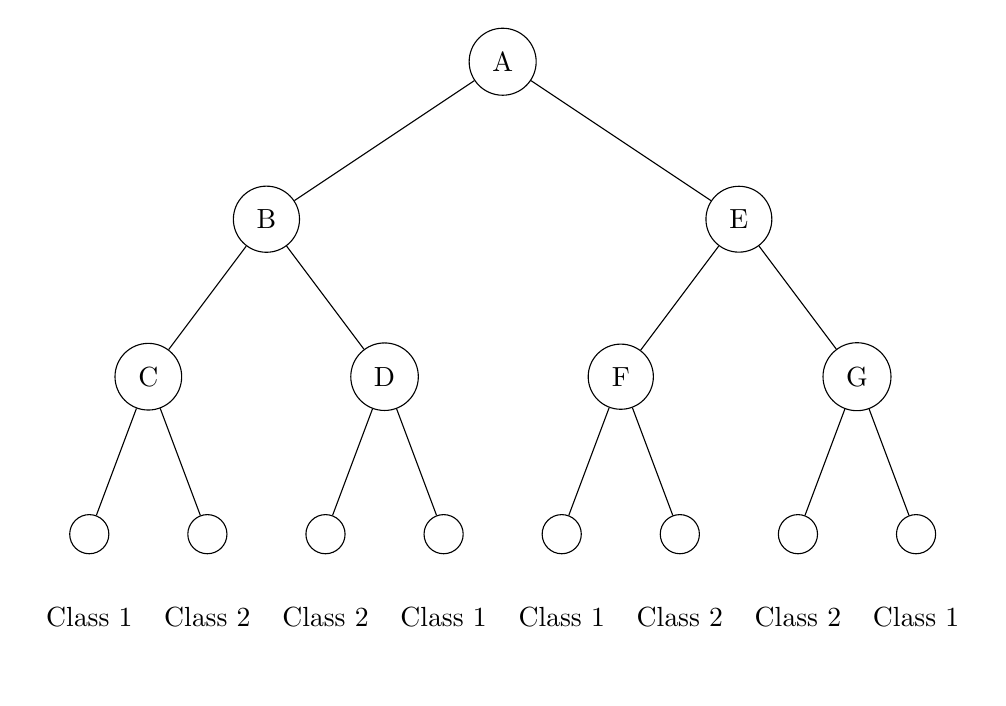
\begin{tikzpicture}[
      grow=down,
      level 1/.style={sibling distance=6cm, level distance=2cm},
      level 2/.style={sibling distance=3cm, level distance=2cm},
      level 3/.style={sibling distance=1.5cm, level distance=2cm},
      every node/.style={draw, circle, inner sep=0.5em}
    ]
    
    % Root node
    \node {A}
      child {
        node {B}
        child {
          node {C}
          child {node[label=below:Class 1] {}}
          child {node[label=below:Class 2] {}}
        }
        child {
          node {D}
          child {node[label=below:Class 2] {}}
          child {node[label=below:Class 1] {}}
        }
      }
      child {
        node {E}
        child {
          node {F}
          child {node[label=below:Class 1] {}}
          child {node[label=below:Class 2] {}}
        }
        child {
          node {G}
          child {node[label=below:Class 2] {}}
          child {node[label=below:Class 1] {}}
        }
      };
    
    \end{tikzpicture}
    \caption{Random Forest}
    \label{fig:rf}
  \end{figure}